%%%%%%%%%%%%%%%%%%%%%%%%%%%%%%%%%%%%%%%%%
% FRI Data Science_report LaTeX Template
% Version 1.0 (28/1/2020)
% 
% Jure Demšar (jure.demsar@fri.uni-lj.si)
%
% Based on MicromouseSymp article template by:
% Mathias Legrand (legrand.mathias@gmail.com) 
% With extensive modifications by:
% Antonio Valente (antonio.luis.valente@gmail.com)
%
% License:
% CC BY-NC-SA 3.0 (http://creativecommons.org/licenses/by-nc-sa/3.0/)
%
%%%%%%%%%%%%%%%%%%%%%%%%%%%%%%%%%%%%%%%%%


%----------------------------------------------------------------------------------------
%	PACKAGES AND OTHER DOCUMENT CONFIGURATIONS
%----------------------------------------------------------------------------------------
\documentclass[fleqn,moreauthors,10pt]{ds_report}
\usepackage[english]{babel}

\graphicspath{{fig/}}




%----------------------------------------------------------------------------------------
%	ARTICLE INFORMATION
%----------------------------------------------------------------------------------------

% Header
\JournalInfo{FRI Natural language processing course 2023}

% Interim or final report
\Archive{Project report} 
%\Archive{Final report} 

% Article title
\PaperTitle{Natural language processing course Latex Template} 

% Authors (student competitors) and their info
\Authors{Aljaž Grdadolnik, Anže Mihevc, and Luka Galjot}

% Advisors
\affiliation{\textit{Advisors: Slavko Žitnik}}

% Keywords
\Keywords{Transformer-Based Language Models, SloBERT, paraphrasing, Transformer-Based Language Models}
\newcommand{\keywordname}{Keywords}


%----------------------------------------------------------------------------------------
%	ABSTRACT
%----------------------------------------------------------------------------------------

\Abstract{
This paper discusses the use of deep learning models, particularly transformer-based language models like BERT, to implement sentence paraphrasing, which is a crucial aspect of natural language processing tasks. The aim is to use a fine-tuned version of SloBERTa to generate paraphrases of sentences by selecting a corpus that includes semantically similar paraphrases while preserving the original meaning. The paper proposes to validate the model using both manual and automatic metrics. The implementation of this approach has the potential to improve the efficiency of natural language processing tasks.
}

%----------------------------------------------------------------------------------------

\begin{document}

% Makes all text pages the same height
\flushbottom 

% Print the title and abstract box
\maketitle 

% Removes page numbering from the first page
\thispagestyle{empty} 

%----------------------------------------------------------------------------------------
%	ARTICLE CONTENTS
%----------------------------------------------------------------------------------------

\section*{Introduction}
	% These latex files are intended to serve as a the template for the NLP course at FRI.  The template is adapted from the FRI Data Science Project Competition. template  If you find mistakes in the template or have problems using it, please consult Jure Demšar (\href{mailto:jure.demsar@fri.uni-lj.si}{jure.demsar@fri.uni-lj.si}).
	
	% In the Introduction section you should write about the relevance of your work (what is the purpose of the project, what will we solve) and about related work (what solutions for the problem already exist). Where appropriate, reference scientific work conducted by other researchers. For example, the work done by Demšar et al. \cite{Demsar2016BalancedMixture} is very important for our project. The abbreviation et al. is for et alia, which in latin means and others, we use this abbreviation when there are more than two authors of the work we are citing. If there are two authors (or if there is a single author) we just write down their surnames. For example, the work done by Demšar and Lebar Bajec \cite{Demsar2017LinguisticEvolution} is also important for successful completion of our project.
Paraphrasing, the process of expressing the same meaning using different words is an important part of natural language processing tasks. Recently, deep learning models, particularly the transformer-based language models like BERT, have achieved remarkable results in several language processing tasks. This paper aims to implement sentence paraphrasing using BERT model, which has demonstrated state-of-the-art performance in range of processing tasks. Specifically we will use fine-tuned version of SloBERTa \cite{11356/1387} to generate paraphrases of sentences. Fine-tuning will be performed by one of the selected corpora, which will be preprocessed to include semantically similar paraphrases while preserving the meaning of the original sentence. We will validate our model with manually defined metrics and automatic methods. 

%------------------------------------------------

\section*{Related work and existing solutions}
Recently with emergence of ChatGPT service many of other companies and academic groups have speed up development of their own LLMs such as GPT-2 (by OpenAI), GPT-3 (by OpenAI), T5 (by Raffel et al. \cite{https://doi.org/10.48550/arxiv.1910.10683}), RoBERTa (by Liu et al. \cite{https://doi.org/10.48550/arxiv.1907.11692}), LLaMa (by Touvron et al. \cite{https://doi.org/10.48550/arxiv.2302.13971}).

In the article \textit{\textbf{The Multilingual Paraphrase Database}}\cite{ganitkevitch2014multilingual} the authors expand their English and Spanish paraphrase database to include 21 other languages including Slovene. They extract the paraphrases from bilingual parallel corpora by “pivoting” words and phrases over a shared translation in another language (English). They make the database freely available. 



%------------------------------------------------

\section*{Initial ideas}
This section aims to provide initial ideas on how to approach the classroom project.

\subsection{Dataset acquisition/generation}
Perhaps the most important part of training a good model for paraphrasing is starting with the right dataset. The dataset should include quality pairs of phrases and their paraphrases. Such datasets already exist mainly for the english language such as The Paraphrase Database (PPDB)\cite{ganitkevitch2013ppdb}. We have found an extended version of PPDB that includes other languages including slovene\cite{ganitkevitch2014multilingual}. Upon further investigation we have determined that the phrases included in this extended database are often only synonyms and the “source” phrases are not longer than 6 words. This dataset was produced using the back translation method or by “pivoting” over a shared translation in another language, in this case english. We would like to see if we get better results using a different method such as automatic translation of non-slovene dataset. We will use a translation model provided in the instructions of this assignment \cite{slovene_nmt} to automatically translate the original PPDB to Slovene. Afterwards we will check the quality and similarity of the translated pairs using different metrics. If our method produced better results than the back translation method we would use the automatically translated dataset to train our paraphrasing model.

More recently the QUORA\cite{sambit7_quora_dataset} and MSCOCO\cite{lin2014microsoft} dataset have been used to train and evaluate paraphrasing models. The QUORA dataset is a dataset of duplicate questions posted on the Quora website. This questions are manually marked by moderators as duplicates so they are confirmed paraphrases. We could use automatic translation to obtain paraphrasing pairs in Slovene. The MSCOCO dataset is not a dataset originally made for paraphrasing or language processing rather it is a dataset of objects and object recognition within images. However the dataset specifically the annotations of the images can still be used to train and test paraphrasing models. To use this model in our assigmnet we would again need to automaticaly translate it and check for the quality of the translated pairs.

\subsection{Natural language deep learning model}
To implement paraphrasing, we can use a deep learning model to fine-tune RoBERTa model on pairs of sentences. The RoBERTa model is a transformer-based model that is pre-trained on a large corpus of text. Fine-tuning the RoBERTa model on pairs of sentences will allow us to train the model to generate paraphrases of the input sentences. The deep learning model will learn to generate paraphrases by minimizing the difference between the predicted paraphrase and the actual paraphrase. This approach has been shown to be effective in generating high-quality paraphrases.

\subsection{Result evaluation}
The quality of the implemented model has to be somehow evaluated so we can compare it to other already existing models. For this we will use different metrics of evaluation. These are BLEU (\textit{Bilingual Evaluation Understudy)} which was developed to evaluate machine translation systems, but can be also used for paragraph evaluation, METEOR which aims to adress BLEU's weakness of being unable to measure semantic equivalents when applied to low-resource languages and has a better correlation with human judgement at the sentence/segment level than BLEU, GLEU, ROUGE a recall-based evaluation metric originally developed for text summarization, has also been used to evaluate paraphrase generation, BERTscore, WER \cite{zhou2021paraphrase}. And lastly we will use human evaluation as a metric, which will probably be the best in scoring, but most definitely the most tidiest and time consuming.

% ROUGE-N and ROUGE-L are mostly used.

%\section*{Methods}


% Use the Methods section to describe what you did an how you did it -- in what way did you prepare the data, what algorithms did you use, how did you test various solutions ... Provide all the required details for a reproduction of your work.

% Below are \LaTeX examples of some common elements that you will probably need when writing your report (e.g. figures, equations, lists, code examples ...).


% \subsection*{Equations}

% You can write equations inline, e.g. $\cos\pi=-1$, $E = m \cdot c^2$ and $\alpha$, or you can include them as separate objects. The Bayes’s rule is stated mathematically as:

% \begin{equation}
% 	P(A|B) = \frac{P(B|A)P(A)}{P(B)},
% 	\label{eq:bayes}
% \end{equation}

% where $A$ and $B$ are some events. You can also reference it -- the equation \ref{eq:bayes} describes the Bayes's rule.

% \subsection*{Lists}

% We can insert numbered and bullet lists:

% % the [noitemsep] option makes the list more compact
% \begin{enumerate}[noitemsep] 
% 	\item First item in the list.
% 	\item Second item in the list.
% 	\item Third item in the list.
% \end{enumerate}

% \begin{itemize}[noitemsep] 
% 	\item First item in the list.
% 	\item Second item in the list.
% 	\item Third item in the list.
% \end{itemize}

% We can use the description environment to define or describe key terms and phrases.

% \begin{description}
% 	\item[Word] What is a word?.
% 	\item[Concept] What is a concept?
% 	\item[Idea] What is an idea?
% \end{description}


% \subsection*{Figures}

% You can insert figures that span over the whole page, or over just a single column. The first one, \figurename~\ref{fig:column}, is an example of a figure that spans only across one of the two columns in the report.

% \begin{figure}[ht]\centering
% 	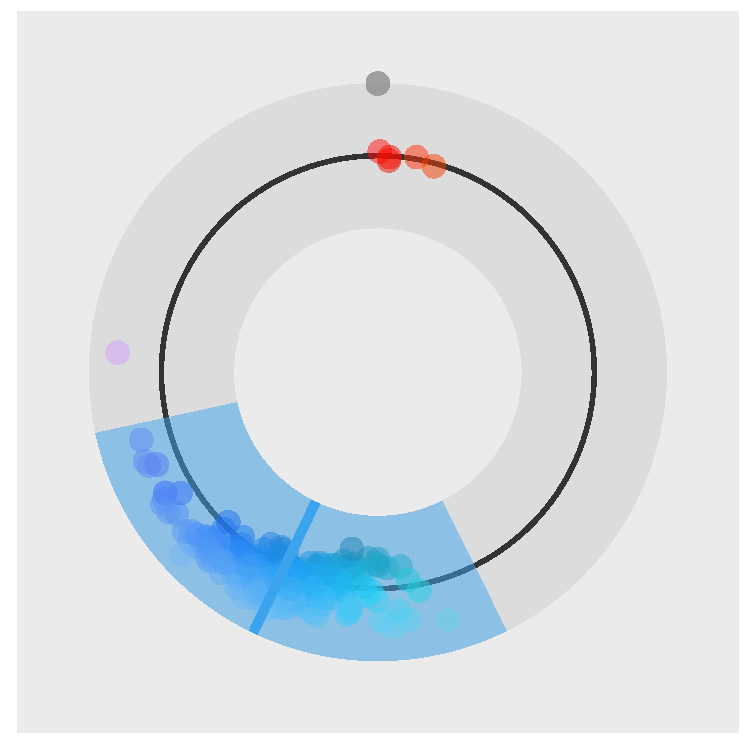
\includegraphics[width=\linewidth]{single_column.pdf}
% 	\caption{\textbf{A random visualization.} This is an example of a figure that spans only across one of the two columns.}
% 	\label{fig:column}
% \end{figure}

% On the other hand, \figurename~\ref{fig:whole} is an example of a figure that spans across the whole page (across both columns) of the report.

% % \begin{figure*} makes the figure take up the entire width of the page
% \begin{figure*}[ht]\centering 
% 	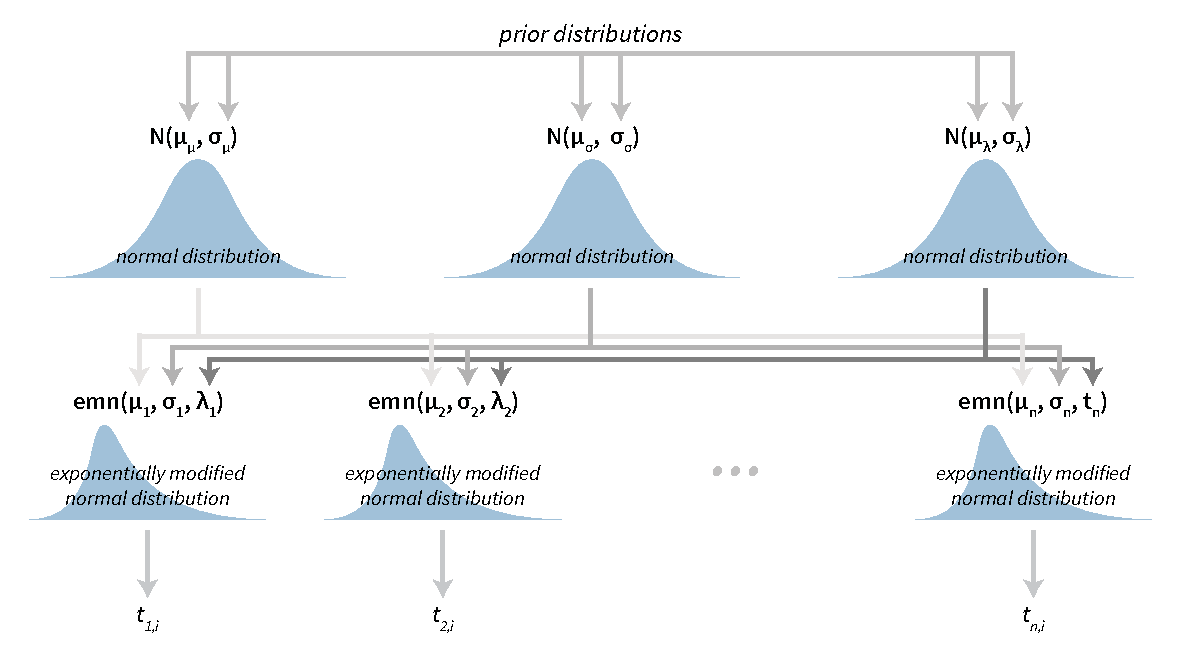
\includegraphics[width=\linewidth]{whole_page.pdf}
% 	\caption{\textbf{Visualization of a Bayesian hierarchical model.} This is an example of a figure that spans the whole width of the report.}
% 	\label{fig:whole}
% \end{figure*}


% \subsection*{Tables}

% Use the table environment to insert tables.

% \begin{table}[hbt]
% 	\caption{Table of grades.}
% 	\centering
% 	\begin{tabular}{l l | r}
% 		\toprule
% 		\multicolumn{2}{c}{Name} \\
% 		\cmidrule(r){1-2}
% 		First name & Last Name & Grade \\
% 		\midrule
% 		John & Doe & $7.5$ \\
% 		Jane & Doe & $10$ \\
% 		Mike & Smith & $8$ \\
% 		\bottomrule
% 	\end{tabular}
% 	\label{tab:label}
% \end{table}


% \subsection*{Code examples}

% You can also insert short code examples. You can specify them manually, or insert a whole file with code. Please avoid inserting long code snippets, advisors will have access to your repositories and can take a look at your code there. If necessary, you can use this technique to insert code (or pseudo code) of short algorithms that are crucial for the understanding of the manuscript.

% \lstset{language=Python}
% \lstset{caption={Insert code directly from a file.}}
% \lstset{label={lst:code_file}}
% \lstinputlisting[language=Python]{code/example.py}

% \lstset{language=R}
% \lstset{caption={Write the code you want to insert.}}
% \lstset{label={lst:code_direct}}
% \begin{lstlisting}
% import(dplyr)
% import(ggplot)

% ggplot(diamonds,
% 	   aes(x=carat, y=price, color=cut)) +
%   geom_point() +
%   geom_smooth()
% \end{lstlisting}

%------------------------------------------------

% \section*{Results}

% Use the results section to present the final results of your work. Present the results in a objective and scientific fashion. Use visualisations to convey your results in a clear and efficient manner. When comparing results between various techniques use appropriate statistical methodology.

% For results we will use different metrics of evaluation. These are BLEU, GLEU, ROUGE, BERTscore, METEOR, WER.


%------------------------------------------------

% \section*{Discussion}

% Use the Discussion section to objectively evaluate your work, do not just put praise on everything you did, be critical and exposes flaws and weaknesses of your solution. You can also explain what you would do differently if you would be able to start again and what upgrades could be done on the project in the future.


%------------------------------------------------

% \section*{Acknowledgments}

% Here you can thank other persons (advisors, colleagues ...) that contributed to the successful completion of your project.


%----------------------------------------------------------------------------------------
%	REFERENCE LIST
%----------------------------------------------------------------------------------------
\bibliographystyle{unsrt}
\bibliography{report}


\end{document}

